%! suppress = EscapeHashOutsideCommand
%! suppress = TooLargeSection
%! suppress = MissingLabel

% * Make friends tikz & colors
%   https://en.wikibooks.org/wiki/LaTeX/Colors
% * To enable vertical top alignment globally
%   https://tex.stackexchange.com/questions/9889/positioning-content-at-the-top-of-a-beamer-slide-by-default
\documentclass[usenames, dvipsnames]{beamer}
% ------------------------------------------------

% Graphics
\usepackage{color}
\usepackage{tabularx}
\usepackage{tikz}
\usepackage{blkarray}
\usepackage{graphicx}
% ------------------------------------------------

% Math
\usepackage{amsmath, amsfonts}
\usepackage{amssymb}
\usepackage{proof}
\usepackage{mathrsfs}
% Crossed-out symbols
% https://tex.stackexchange.com/questions/75525/how-to-write-crossed-out-math-in-latex
\usepackage[makeroom]{cancel}
\usepackage{mathtools}
% ------------------------------------------------

% Additional font sizes
% https://www.overleaf.com/learn/latex/Questions/How_do_I_adjust_the_font_size%3F
\usepackage{moresize}
% Additional colors
% https://www.overleaf.com/learn/latex/Using_colours_in_LaTeX
\usepackage{xcolor}
% ------------------------------------------------

% Language
\usepackage[utf8] {inputenc}
\usepackage[T2A] {fontenc}
\usepackage[english, russian] {babel}
\usepackage{indentfirst, verbatim}
\usetikzlibrary{cd, babel}
% ------------------------------------------------

% Fonts
\usepackage{stmaryrd}
\usepackage{cmbright}
\usepackage{wasysym}
% ------------------------------------------------

% Code
% https://tex.stackexchange.com/questions/99475/how-to-invoke-latex-with-the-shell-escape-flag-in-texstudio-former-texmakerx
\usepackage{minted}
\setminted{xleftmargin=\parindent, autogobble, escapeinside=\#\#}
% ------------------------------------------------

% Template
\usetheme{CambridgeUS}
\usecolortheme{dolphin}
% https://tex.stackexchange.com/questions/231439/beamer-how-to-make-font-larger-for-page-numbers
\setbeamerfont{headline}{size=\scriptsize}
\setbeamerfont{footline}{size=\scriptsize}
% Remove heddline
% https://tex.stackexchange.com/questions/33146/how-could-i-remove-a-header-in-a-beamer-presentation
%\setbeamertemplate{headline}{}
% Slide sizes
% https://tex.stackexchange.com/questions/56768/how-to-set-a-small-default-font-size-with-beamer
%\geometry{paperwidth=140mm,paperheight=105mm} % 4:3
\geometry{paperwidth=168mm,paperheight=105mm} % 16:10
% Remove navigation bar
% https://stackoverflow.com/questions/3210205/how-to-get-rid-of-navigation-bars-in-beamer
\beamertemplatenavigationsymbolsempty
% ------------------------------------------------

% Bullets
% https://9to5science.com/change-bullet-style-formatting-in-beamer
% https://tex.stackexchange.com/questions/185742/i-need-to-change-color-of-beamer-itemize-and-subitem-separately
\setbeamertemplate{itemize item}{\scriptsize\raise1.25pt\hbox{\donotcoloroutermaths$\blacktriangleright$}}
\setbeamertemplate{itemize subitem}{\tiny\raise1.5pt\hbox{\donotcoloroutermaths$\blacktriangleright$}}
\setbeamertemplate{itemize subsubitem}{\tiny\raise1.5pt\hbox{\donotcoloroutermaths$\blacktriangleright$}}
\setbeamertemplate{enumerate item}{\insertenumlabel.}
\setbeamertemplate{enumerate subitem}{\insertenumlabel.\insertsubenumlabel}
\setbeamertemplate{enumerate subsubitem}{\insertenumlabel.\insertsubenumlabel.\insertsubsubenumlabel}
% ------------------------------------------------

% Table of contents format
% https://tex.stackexchange.com/questions/642927/format-table-of-contents-in-beamer
\setbeamertemplate{section in toc}{%
        {\color{blue}\inserttocsectionnumber.}
    \inserttocsection\par%
}
\setbeamertemplate{subsection in toc}{%
        {\color{blue}\hspace{1em}\scriptsize\raise1.25pt\hbox{\donotcoloroutermaths$\blacktriangleright$}}
    \inserttocsubsection\par%
}
\setbeamertemplate{subsubsection in toc}{%
        {\color{blue}\hspace{2em}\tiny\raise1.25pt\hbox{\donotcoloroutermaths$\blacktriangleright$}}
    \inserttocsubsubsection\par%
}
% ------------------------------------------------

% Diff
\usepackage{multicol}
\usepackage{hyperref}
\usepackage{soul} % https://tex.stackexchange.com/questions/23711/strikethrough-text
% ------------------------------------------------

% Appendix
% Slide numbers
% https://tex.stackexchange.com/questions/70448/dont-count-backup-slides
\usepackage{appendixnumberbeamer}
\newcommand{\backupbegin}{
    \newcounter{framenumbervorappendix}
    \setcounter{framenumbervorappendix}{\value{framenumber}}
}
\newcommand{\backupend}{
    \addtocounter{framenumbervorappendix}{-\value{framenumber}}
    \addtocounter{framenumber}{\value{framenumbervorappendix}}
}
% ------------------------------------------------

% Custom commands
\newcommand{\err}[0]{\textcolor{red}{ошибка}}
% ------------------------------------------------

% Speaker notes
% https://tex.stackexchange.com/questions/114219/add-notes-to-latex-beamer
% https://tex.stackexchange.com/questions/35444/split-beamer-notes-across-multiple-notes-pages/35496#35496
\setbeameroption{show notes on second screen=right} % enable speaker notes
%--------------------------------------

\author[Андрей Стоян]{Стоян Андрей Сергеевич \\ {\footnotesize научный руководитель: к.~ф.-м.~н.} Москвин Денис Николаевич \\ {\footnotesize научный консультант:} Новожилов Дмитрий Павлович}
\institute[ИТМО/SE]{Университет ИТМО\\Разработка программного обеспечения/Software engineering}

\title[Self-типы для языка Kotlin]{Дизайн и разработка Self-типов для языка Kotlin}
\date{Санкт-Петербург 2023г.}

\begin{document}
    \setcounter{framenumber}{-1}

    \maketitle
    \note{
        0 - 0:20

        \begin{enumerate}
            \item Добрый день!
            \item Меня зовут Стоян Андрей
            \item Тема моей дипломной работы: дизайн и разработка Self-типов для языка Kotlin
            \item Научный руководитель: Москвин Денис Николаевич
            \item Научный консультант: Новожилов Дмитрий Павлович
        \end{enumerate}
    }


    \section{Введение}


    \subsection{Предметная область}

    \begin{frame}{Системы типов}
        \note{
            0:20 - 0:40

            \begin{enumerate}
                \item Анализ типов позволяет выявлять заведомо некорректны программы
                \begin{enumerate}
                    \item но в то же время не допускает много корректных
                \end{enumerate}
                \item Поэтому задачи дизайна безопасной системы типов для промышленного языка можно сформулировать следующим образом:
                \begin{enumerate}
                    \item во-первых, отвергнуть все некорректные программы
                    \item во-вторых типизировать как можно больше корректных программ
                    \item но при этом не увеличить чрезмерно сложность и многословность кода
                \end{enumerate}
            \end{enumerate}
        }

        \begin{itemize}
            \item Система типов позволяет выявлять заведомо некорректные программы
            \item Проверка нетривиальных свойств программы --- неразрешимая задача
            \item Анализ типов отвергает много корректных программ, чтобы оставаться разрешимым
        \end{itemize}

        \begin{center}
            \includegraphics[width=0.36\textwidth]{fig/types}
        \end{center}

        \begin{block}{Задачи дизайна безопасной системы типов для промышленного языка программирования}
            \begin{itemize}
                \item Отвергнуть все некорректные программы (с точки зрения типов времени исполнения)
                \item Типизировать как можно больше корректных программ без потери практичности:
                \begin{itemize}
                    \item Сложность понимания
                    \item Многословность кода
                \end{itemize}
            \end{itemize}
        \end{block}
    \end{frame}


    \subsection{Постановка проблемы}

    \begin{frame}[fragile]{Ограничение текущей системы типов Kotlin}
        \note{
            0:40 - 1:10

            \begin{enumerate}
                \item На данный момент в системе типов Kotlin нет прямого способа записать тип получателя
                \begin{enumerate}
                    \item То есть тип объекта, на котором вызывается метод
                \end{enumerate}
                \item Это приводит к нехватке точности анализа типов, а именно полезный корректный код не типизируется
                \begin{enumerate}
                    \item Так в примере метод добавления элемента в персистентную коллекцию, очевидно, возвращает новую коллекцию того же типа, на которой он вызван
                    \item Однако мы не можем написать в декларации тип специфичнее базового
                    \item Поэтому его и возвращает вызов метода add на наследнике
                    \item Что приводит и к ошибке типизации в данном коде, несмотря на его корректность
                \end{enumerate}
            \end{enumerate}
        }

        \begin{block}{Ограничение}
            Нет прямого способа написать тип получателя\footnote{\emph{Получатель вызова} --- объект, на котором вызывается метод. Пример: \mintinline{kotlin}|a.f()|, \texttt{a} --- получатель.} (\mintinline{kotlin}|this|'а) в декларации метода.
        \end{block}

        \begin{block}{Нехватка точности анализа типов (корректный код не типизируется)}
            \begin{minted}{kotlin}
                interface PCollection<E> {
                    fun add(elem: E): #\framebox{PCollection<E>}# // нет способа написать тип специфичнее
                }
                fun test(list: PList<Int>) {
                    list.add(42)        // : #\framebox{PCollection<Int>}# - базовый тип
                        .listSpecific() // #\textcolor{red}{ошибка типизации}#
                }
            \end{minted}
        \end{block}
    \end{frame}


    \subsection{Существующие решения}

    \begin{frame}[fragile]{Существующие способы записи типа получателя}
        \note{
            1:10 - 1:40

            \begin{enumerate}
                \item Способы записать тип получателя всё же существуют
                \item Первый вариант --- добавить типовой параметр с рекурсивным ограничением
                \begin{enumerate}
                    \item Он небезопасный и сложный
                    \item А так же многословный: дополнительный типовой параметр распространяется по всему коду
                \end{enumerate}
                \item Второй вариант --- добавить переопределяющие методы с более специфичным возвращаемым типом
                \begin{enumerate}
                    \item Этот вариант многословный и работает только для возвращаемых типов
                \end{enumerate}
                \item И третий вариант --- ассоциированные типы, который, в отличие от предыдущих двух, не доступен в Kotlin, но доступен, например, в Scala
                \begin{enumerate}
                    \item Помимо прочих недостатков, сложен в использовании и реализации
                \end{enumerate}
            \end{enumerate}
        }

        \begin{block}{Типовой параметр с рекурсивным ограничением (Kotlin)}
            \mintinline{kotlin}|interface PCollection<E, #\framebox{S : PCollection<E, S>}#>|
            \begin{itemize}
                \item[$\color{red} -$] Небезопасность: явное приведение типов: \mintinline[escapeinside=??]{kotlin}|this as S|
                \item[$\color{red} -$] Сложность: рекурсивное ограничение
                \item[$\color{red} -$] Многословность: дополнительный типовой параметр распространяется по всему коду
%                \item[$-$] Зафиксированный типовой аргумент \texttt{S} не может быть уточнён в наследниках
            \end{itemize}
        \end{block}

        \begin{block}{Переопределяющие методы с более специфичным возвращаемым типом (Kotlin)}
            \begin{itemize}
                \item[$\color{red} -$] Ненадёжность: нет контроля компилятора, что такие методы не были забыты
                \item[$\color{red} -$] Многословность: переопределить каждый метод в каждом наследнике
                \item[$\color{red} -$] Ограниченность: только для возвращаемого типа
            \end{itemize}
        \end{block}

        \begin{block}{Ассоциированные типы (Scala)}
            \begin{itemize}
                \item[$\color{red} -$] Небезопасность, ненадёжность, ограниченность
                \item[$\color{red} -$] Сложность использования и реализации [\href{http://lampwww.epfl.ch/~amin/dot/fpdt_post.pdf}{Path-dependent types, Odersky et al, 2014}]
            \end{itemize}
        \end{block}
    \end{frame}

    \begin{frame}[fragile]{Self-типы}
        \note{
            1:40 - 2:10

            \begin{enumerate}
                \item Прямым способом записи типа получателя являются Self-типы
                \begin{enumerate}
                    \item они не имеют недостатков своих альтернатив
                    \item однако требуют нетривиального языкового дизайна
                \end{enumerate}
                \item Так, нужно просто вернуть Self-тип в методе add базового интерфейса
                \begin{enumerate}
                    \item и теперь на его результате можно вызывать методы наследника
                    \item то есть этот код уже проходит проверку типов
                \end{enumerate}
            \end{enumerate}
        }

        \begin{itemize}
            \item[$\Delta$] \emph{Self-тип} --- прямой способ записи типа получателя вызова (тип \mintinline{kotlin}|this|'а)
            \item[$+$] Не имеет упомянутых ранее недостатков
            \item[$\color{red} -$] Требует нетривиального языкового дизайна
        \end{itemize}

        \begin{block}{Self-типы уточняют анализ типов}
            \begin{minted}{kotlin}
                interface PCollection<out E> {
                    fun add(value: E): #\framebox{Self}#
                }
                fun test(list: PList<Int>) {
                    list.add(x)         // область видимости #\framebox{PList<Int>}#
                        .listSpecific() // корректный код типизируется
                }
            \end{minted}
        \end{block}
    \end{frame}


    \section{Цель и задачи}

    \begin{frame}{Цель и задачи}
        \note{
            2:10 - 2:40

            \begin{enumerate}
                \item Таким образом, цель моей работы ---
                \item Разработать дизайн Self-типов для языка Kotlin на основании опыта других языков и реализовать поддержку Self-типов в компиляторе kotlinc.
                \item Для этого нужно выделить особенности существующих решений, такие как:
                \begin{enumerate}
                    \item возможные значения Self-типа
                    \item допустимые позиции Self-типа
                    \item и меры по обеспечению безопасности системы типов
                \end{enumerate}
                \item Затем интегрировать Self-типы в типовую систему языка Kotlin на основании проведённого анализа решений
                \item И наконец, реализовать поддержку Self-типов в компиляторе kotlinc
            \end{enumerate}
        }

        \begin{block}{Цель}
            Разработать дизайн Self-типов для языка Kotlin на основании опыта других языков и реализовать поддержку Self-типов в компиляторе kotlinc.
        \end{block}

        \begin{block}{Задачи}
            \begin{enumerate}
                \item Выделить особенности существующих решений: возможные значения Self-типа, допустимые позиции Self-типа и меры по обеспечению безопасности системы типов
                \item Интегрировать Self-типы в типовую систему языка Kotlin на основании проведённого анализа решений
                \item Реализовать поддержку Self-типов в компиляторе kotlinc
            \end{enumerate}
        \end{block}
    \end{frame}


    \section{Ход работы}


    \subsection{Существующие решения}

    \begin{frame}{Существующие реализации Self-типов}
        \note{
            2:40 - 3:10

            \begin{enumerate}
                \item Рассмотрим существующие реализации Self-типов
                \item В научных работах используется типизированное лямбда исчисление
                \begin{enumerate}
                    \item где на простой модели становятся видны как тонкие места, в которых система может стать небезопасной,
                    \item так и возможные решения таких проблем
                \end{enumerate}
                \item Во многих прикладных языках же реализация Self-типов небезопасна: Python, TS и Java с плагином
                \item Однако Swift же имеет полноценную безопасную поддержку
                \item Далее я интегрирую Self-типы в типовую систему языка Kotlin, опираясь как на академические результаты, так и на реализацию в Swift
            \end{enumerate}
        }

        \begin{block}{Академические результаты, характерные черты}
            \begin{itemize}
                \item Кодирование в типизированном лямбда-исчислении
                \item Видны места потенциального нарушения безопасности системы типов
                \item Предлагаются наиболее гибкие решения, нередко в ущерб практичности
%                \item Видны аспекты сохранения безопасности системы с Self-типами
%                \item Свойства результатов доказываются на модельных исчислениях [\href{https://dl.acm.org/doi/pdf/10.1145/503502.503505}{FJ}, \href{https://dl.acm.org/doi/pdf/10.1145/2888392}{CoreThisJava}]
            \end{itemize}
        \end{block}

        \begin{block}{Прикладные языки, поддерживающие Self-типы}
            \begin{itemize}
                \item[$\color{red} \mathbf{\times}$] Python, TypeScript, Java с плагином Manifold --- небезопасная реализация
                \item[$\color{red} \mathbf{\times}$] Rust не поддерживает нетривиальные случаи использования Self-типов % запрещено создавать трейт-объект\footnote{Трейты --- механизм специального полиморфизма в Rust}\footnote{Трейт-объект --- способ использовать неизвестный тип, реализующий трейт: \mintinline{rust}|Box<dyn Trait>|} при наличии метода с Self-типом
                \item Swift --- полноценная безопасная реализация Self-типов
            \end{itemize}
        \end{block}
    \end{frame}


    \subsection{Интеграция Self-типов в типовую систему языка Kotlin}

    \begin{frame}[fragile]{Переписывание Self-типа}
        \note{
            3:10 - 3:50

            \begin{enumerate}
                \item Сначала я заметил, что Self-типу небезопасно покидать контекст своего объекта
                \begin{enumerate}
                    \item Так, если пример слева проходит проверку типов
                    \item То объект типа A на выходе метода unsafe получает область видимости наследника
                    \item Что может привести к ошибке времени исполнения
                \end{enumerate}
                \item Однако можно заметить, что Self-тип аналогичен параметру рекурсивного типа
                \item А чтобы воспользоваться его значением, нужно применить правило развёртки
                \item Я адаптировал его для Kotlin следующим образом:
                \begin{enumerate}
                    \item Self-тип переписывается в тип получателя в его области видимости
                    \item Теперь код в рамке имеет тип A
                    \item И если никакой другой тип не будет являться подтипом Self-типа
                    \item То небезопасный код слева больше не будет типизироваться
                \end{enumerate}
            \end{enumerate}
        }

        \vspace{-1.5em}
        \begin{columns}[onlytextwidth]
            \begin{column}[t]{0.485\textwidth}
                \begin{block}{Пример: небезопасность покидания Self-типом контекста объекта}
                    \begin{minted}{kotlin}
                        open class A {
                            fun self(): Self = this
                            fun unsafe(a: A): Self = #\framebox{a.self()}#
                        }

                        class B : A() {
                            fun bOnly() {}
                        }

                        fun test(b: B) {
                            val a = A()
                            b.unsafe(a) // область видимости B
                             .bOnly()   // #\textcolor{red}{ошибка исполнения}#
                        }
                    \end{minted}
                \end{block}
            \end{column}\hfill%
            \begin{column}[t]{0.485\textwidth}
                \begin{block}{Академическое решение}
                    \begin{itemize}
                        \item Self-тип аналогичен параметру рекурсивного типа $\mu Self\ldotp T[Self]$
                        \item Для использования требуется применить правило развертки (unfold)
                    \end{itemize}
                \end{block}
                \begin{block}{Решение для Kotlin}
                    \begin{itemize}
                        \item Self-тип должен переписываться в тип получателя в его области видимости:
                        \[(self : A.() \to \framebox{$A$}) \in scope(A)\]
                        \item Ограничение подтипизации: \[\forall T \ldotp T \bcancel{<:} Self, T \neq \bot, T \neq Self\]
                    \end{itemize}
                    \vspace{0.23em}
                \end{block}
            \end{column}
        \end{columns}
    \end{frame}

    \begin{frame}[fragile]{Значения Self-типа: существующие решения}
        \note{
            3:50 - 4:20

            \begin{enumerate}
                \item Для приложений важно уметь безопасно типизировать посторонние объекты Self-типом
                \item Академические решения предлагают для этого введение специальных видов методов
                \begin{enumerate}
%                    \item Однако они затрудняют дальнейшее развитие языка --- их придётся далее специальным образом учитывать
                    \item Они усложняют язык
                    \item И их непросто использовать из-за множества сопутствующих нетривиальных правил
                \end{enumerate}
                \item А в прикладных языках вовсе не поддерживается типизация посторонних объектов Self-типом
                \item несмотря на наличие у этого важных приложений
            \end{enumerate}
        }

        \begin{block}{Академические решения}
            \begin{itemize}
                \item Специальные виды методов с безопасной типизацией посторонних объектов Self-типом
                \begin{itemize}
                    \item Ненаследуемые методы\footnote{Не могут быть унаследованы --- требуют переопределение в каждом наследнике} [\href{http://www.fos.kuis.kyoto-u.ac.jp/~igarashi/papers/pdf/thistype-SAC09.pdf}{Saito et al, 2009}]
                    \item Виртуальные конструкторы\footnote{Могут быть унаследованы по сложным правилам} [\href{https://www.researchgate.net/profile/Sukyoung-Ryu/publication/254004584_Exact_type_parameterization_and_ThisType_support/links/54b90ed10cf269d8cbf72d01/Exact-type-parameterization-and-ThisType-support.pdf}{Na et al, 2012}]
                \end{itemize}
%                \item[$\color{red} -$] Затрудняется последующее развитие языка
                \item[$\color{red} -$] Усложняют язык: новая сущность
                \item[$\color{red} -$] Непросто использовать: рутинный код и нетривиальные правила
            \end{itemize}
        \end{block}

        \begin{block}{Решения в прикладных языках}
            \begin{itemize}
                \item Только объект получатель (\mintinline{kotlin}|this|) имеет Self-тип
                \begin{itemize}
                    \item[$\Rightarrow$] Нельзя создавать новые объекты Self-типа
                    \item[$\color{red} -$] Необходимо для важных приложений (например, персистентные коллекции)
                \end{itemize}
            \end{itemize}
        \end{block}
    \end{frame}

    \begin{frame}[fragile]{Значения Self-типа: решение для Kotlin}
        \note{
            4:20 - 4:50

            \begin{enumerate}
                \item Чтобы всё-таки поддержать в Kotlin безопасную типизацию посторонних объектов Self-типом
                \item Я сформулировал следующее условие:
                \begin{enumerate}
                    \item Тип C может быть безопасно заменён на Self-тип, если можно показать статически, что он подтип любого возможного типа получателя
                \end{enumerate}
                \item Это условие я аппроксимировал следующим правилом:
                \begin{enumerate}
                    \item Класс C должен быть финальныи,
                    \item а тип получателя либо равен C, либо включает его после смарткаста
%                    \item Так же должны совпадать модули деклараций, чтобы гарантировать обратную совместимость исходных кодов при открытии класса
                \end{enumerate}
                \item Это правило просто использовать, как показано на примере справа
                \item Но оно имеет ограниченную поддержку открытых классов
            \end{enumerate}
        }

        \begin{block}{Условие безопасной замены типа \texttt{C} на \texttt{Self}}
            \mintinline{kotlin}|C::class isSubtypeOf this.getClass()| должно выполняться статически
        \end{block}

%        \vspace{-1.5em}
        \begin{columns}[onlytextwidth]
            \begin{column}{0.485\textwidth}
                \begin{block}{Правило значений Self-типа для Kotlin}
                    \begin{enumerate}
                        \item Класс \texttt{C} должен быть финальным
                        \item Тип \mintinline{kotlin}|this|
%                        \footnote{Получатель вызова текущей декларации}
                        либо равен \texttt{С}, либо включает \texttt{C} после smart-cast
                        \item Тип \texttt{C} объявлен в том же модуле, в котором создаётся объект
%                        \footnote{Иначе открытие класса нарушает совместимость исходных кодов}
                    \end{enumerate}
                \end{block}
                \begin{block}{}
                    \begin{itemize}
                        \item[$+$] Простота использования
                        \item[$\color{red} -$] Ограниченная поддержка открытых классов
                    \end{itemize}
                \end{block}
            \end{column}\hfill%
            \begin{column}{0.485\textwidth}
                \begin{block}{Пример: персистентный список}
                    \begin{minted}{kotlin}
                        class PListImpl<E> : PList<E> {
                            override fun add(elem: E): Self {
                                val newList = Cons(elem, list)
                                return #\framebox{PListImpl(newList)}#
                            }
                        }
                    \end{minted}
                \end{block}
            \end{column}
        \end{columns}
    \end{frame}

    \begin{frame}[fragile]{Возможные позиции Self-типа: ковариантные позиции}
        \note{
            4:50 - 5:10

            \begin{enumerate}
                \item Рассмотрим возможные позиции Self-типа
                \item Известно, что Self-типы можно безопасно использовать в ковариантных позициях
                \item Однако Swift поддерживает только позицию возвращаемого типа
                \item Но у Kotlin, в отличие, от Swift есть поддержка вариантности типовых параметров
                \item Поэтому допустимо использовать Self-типы в том числе в позициях типовых аргументов
            \end{enumerate}
        }

        \begin{block}{Ковариантные позиции --- значение передаётся вызывающему коду}
            \begin{itemize}
                \item \mintinline{kotlin}|fun add(elem: E): #\framebox{Self}#| % из \mintinline{kotlin}|interface PCollection<out E>|
                \item \mintinline{kotlin}|fun onClick(observer: (#\framebox{Self}#) -> Unit)| % из \mintinline{kotlin}|abstract class BaseButton|
            \end{itemize}
        \end{block}

        \begin{block}{Академический результат}
            \begin{itemize}
                \item Self-типы можно безопасно использовать в ковариантных позициях~[\href{https://dl.acm.org/doi/pdf/10.1145/96709.96721}{Cook et al, 1989}]
            \end{itemize}
        \end{block}

        \begin{block}{Решение в Swift}
            \begin{itemize}
                \item Нет поддержки вариантности типовых параметров
                \item Полностью разрешена только позиция возвращаемого типа
            \end{itemize}
        \end{block}

        \begin{block}{Решение для Kotlin}
            \begin{itemize}
                \item Есть поддержка вариантности типовых параметров
                \item Допустимо использовать Self-типы во всех ковариантных позициях
            \end{itemize}
        \end{block}
    \end{frame}

    \begin{frame}[fragile]{Контравариантные позиции Self-типа: существующие решения}
        \note{
            5:10 - 5:30

            \begin{enumerate}
                \item Назовём сложными методы, которые содержат Self-типы в контравариантной позиции
                \item Известно, что если в классе есть сложный метод, то его наследник не является его подтипом
                \item Поэтому научные работы предлагают существенные ограничения для таких методов
                \item А так же вводят массивные изменения в системе типов для расширения их небольших возможностей
%                \item В Swift запрещено делать виртуальный вызов сложного метода
            \end{enumerate}
        }

        \begin{block}{Контравариантные позиции --- значение передаётся коду метода}
            \begin{itemize}
                \item[$\Delta$] \emph{Сложные методы} --- методы, содержащие Self-тип в контравариантной позиции
                \item \mintinline{kotlin}|fun combine(other: #\framebox{Self}#): Self| % из \mintinline{kotlin}|interface Semigroup|
            \end{itemize}
        \end{block}

        \begin{block}{Академические результаты}
            \begin{itemize}
                \item В классе есть сложный метод $\Rightarrow$ наследник не является подтипом~[\href{https://dl.acm.org/doi/pdf/10.1145/96709.96721}{Cook et al, 1989}]
                \begin{itemize}
                    \item Отношение matching'а вместо подтипизации [\href{https://www.researchgate.net/profile/Kim-Bruce-2/publication/221496196_Subtyping_Is_Not_a_Good_Match_for_Object-Oriented_Languages/links/09e415122545c6d7a4000000/Subtyping-Is-Not-a-Good-Match-for-Object-Oriented-Languages.pdf}{Bruce et al, 1996}]
                    \item Разделение точных и экзистенциальных типов, локальное уточнение [\href{http://www.fos.kuis.kyoto-u.ac.jp/~igarashi/papers/pdf/thistype-SAC09.pdf}{Saito et al, 2009}]
                    \item Именованные wildcard'ы и точные типовые параметры [\href{https://www.researchgate.net/profile/Sukyoung-Ryu/publication/254004584_Exact_type_parameterization_and_ThisType_support/links/54b90ed10cf269d8cbf72d01/Exact-type-parameterization-and-ThisType-support.pdf}{Na et al, 2012}]
                \end{itemize}
                \item[$\color{red} -$] Специальные правила ограничивают использование сложных методов
                \item[$\color{red} -$] Массивные изменения в системе типов для больших возможностей
            \end{itemize}
        \end{block}

        \begin{block}{Решение в Swift}
            \begin{itemize}
                \item Запрещено делать виртуальный вызов сложного метода
            \end{itemize}
        \end{block}
    \end{frame}

    \begin{frame}[fragile]{Контравариантные позиции Self-типа: решение для Kotlin}
        \note{
            5:30 - 6:00

            \begin{enumerate}
                \item Для поддержания сложных методов для них так или иначе запрещают виртуальную диспетчеризацию
                \item поэтому вместо неё можно использовать статическую в виде эмуляции классов типов
                \item это можно сделать через контексты языка Kotlin, как я показал на примере
                \item А значит, другая возможность языка покрывает сценарии использования сложных методов
                \item Поэтому, я предложил запретить использование Self-типов в контравариантных позициях в Kotlin
            \end{enumerate}
        }

        \begin{itemize}
            \item Для поддержки сложных методов запрещают виртуальную диспетчеризацию на них
            \item[$\Rightarrow$] Можно использовать статическую, эмулируя классы типов в Kotlin
            \item[$\Rightarrow$] Другая возможность языка покрывает сценарии использования сложных методов
        \end{itemize}

        \begin{block}{Эмуляция трейтов с помощью контекстов языка Kotlin}
            \begin{minted}{kotlin}
                interface Semigroup<S> {
                    fun S.combine(other: S): S
                }

                context(Semigroup<S>)
                fun <S> combineAll(xs: Iterable<S>): S =
                    xs.reduce { acc, x -> acc.combine(x) }
            \end{minted}
        \end{block}

        \begin{block}{Решение для Kotlin}
            Запрет на использование Self-типов в контравариантных позициях.
        \end{block}
    \end{frame}


    \subsection{Реализация поддержки Self-типов в компиляторе kotlinc}

    \begin{frame}[fragile]{Реализованная функциональность}
        \note{
            6:00 - 6:30

            \begin{enumerate}
                \item В прототипе системы с Self-типами в компиляторе kotlinc я подержал:
                \begin{enumerate}
                    \item Использование Self-типов в ковариантных позициях
                    \item Типизацию посторонних объектов Self-типом
                    \item А так же проверку на использование Self-типов в недопустимых позициях
                \end{enumerate}
            \end{enumerate}
        }

        \begin{block}{Ковариантные позиции Self-типа}
            \begin{minted}{kotlin}
                interface Button {
                    fun onClick(observer: (#\framebox{Self}#) -> Unit)
                }
                checkBox.onClick { print(#\framebox{it}#.isChecked) }
            \end{minted}
        \end{block}
        \begin{block}{Типизация посторонних объектов Self-типом}
            \begin{minted}{kotlin}
                class PListImpl<E> : PList<E> {
                    override fun add(elem: E): #\framebox{Self}# = #\framebox{PListImpl}#(/*...*/)
                }
            \end{minted}
        \end{block}
        \begin{block}{Реализована проверка на использование Self-типов в недопустимых позициях}
            \begin{minted}{kotlin}
                class Semigroup {
                    fun combine(other: #\framebox{Self}#) // ошибка компиляции
                }
            \end{minted}
        \end{block}
    \end{frame}


    \section{Результаты}

    \begin{frame}{Результаты}
        \note{
            6:30 - 7:00

            \begin{enumerate}
                \item Таким образом, в данной работе
                \item Были проанализированы существующие реализации Self-типов | на предмет их возможностей и предлагаемых мер по обеспечению безопасности системы с Self-типами
                \item Self-типы были интегрированы в типовую систему языка Kotlin с опорой на существующие решения
                \item А так же прототип системы с Self-типами был реализован в компиляторе kotlinc
                \item Спасибо за внимание!
            \end{enumerate}
        }

        \begin{enumerate}
            \item Проанализированы существующие реализации Self-типов в других языках на предмет их возможностей и мер по обеспечению безопасности системы с Self-типами
            \item Self-типы интегрированы\footnote{\url{https://github.com/winter-yuki/kotlin-self-types}} в типовую систему языка Kotlin с опорой на существующие решения
            \item Прототип системы с Self-типами реализован\footnote{\url{https://github.com/winter-yuki/kotlin/tree/self-types}} в компиляторе kotlinc
        \end{enumerate}
    \end{frame}


    \appendix


    \section*{Дополнительные слайды}

    \begin{frame}{Содержание дополнительных слайдов}
        \tableofcontents
    \end{frame}


    \subsection{Материалы}

    \begin{frame}{Материалы}
        %! suppress = LineBreak
        \begin{enumerate}
            \item \href{https://youtrack.jetbrains.com/issue/KT-6494}{\color{blue} YouTrack: Запрос на добавление Self-типов в Kotlin}
            \item Cook, William R., Walter Hill, and Peter S. Canning. 1989. <<Inheritance is not subtyping>>. Proceedings of the 17th ACM SIGPLAN-SIGACT symposium on Principles of programming languages. {\color{blue}\url{https://cs.rice.edu/~javaplt/papers/Inheritance.pdf}}
            \item Sukyoung Ryu. 2016. <<ThisType for Object-Oriented Languages: From Theory to Practice>>. ACM Trans. Program. Lang. Syst. 38, 3, Article 8 (May 2016), 66 pages. {\color{blue}\url{https://dl.acm.org/doi/10.1145/2888392}}
            \item \href{https://github.com/manifold-systems/manifold/blob/master/manifold-deps-parent/manifold-ext/README.md\#the-self-type-with-self}{\color{blue} Self-типы как плагин для Java}
            \item \href{https://docs.swift.org/swift-book/documentation/the-swift-programming-language/types/\#Self-Type}{\color{blue} Swift: Self-типы}
            \item \href{https://peps.python.org/pep-0673/}{\color{blue} Python: Self-типы PEP}
            \item \href{https://www.typescriptlang.org/docs/handbook/2/classes.html\#this-types}{\color{blue}TypeScript: this-типы}
        \end{enumerate}
    \end{frame}


    \subsection{Kotlin}

    \begin{frame}[fragile]{Ресиверы (получатели) в Kotlin}
        %! suppress = Quote
        \begin{block}{(Dispatch) Ресивер функции}
            Специальный параметр функции, по которому происходит виртуальная диспетчеризация вызова к реализации наследника.
            Доступен как \mintinline{kotlin}|this| в её теле.
            \begin{itemize}
                \item Например, в вызове \mintinline{kotlin}|"a".plus("b")| строка \mintinline{kotlin}|"a"| является ресивером для функции \mintinline{kotlin}|plus|
            \end{itemize}
        \end{block}
        \pause
        \begin{block}{Область видимости типа}
            Множество функций, для которых объект данного типа может быть использован как ресивер.
            \begin{itemize}
                \item Функция \mintinline{kotlin}|plus| содержится в области видимости типа \mintinline{kotlin}|String|: \\
                \mintinline{kotlin}|(plus: String.(String) -> String)| $\in$ \mintinline{kotlin}|scope(String)|
            \end{itemize}
        \end{block}
    \end{frame}

    \begin{frame}{Вариантность}
        \begin{block}{Вариантность типового параметра}
            \begin{itemize}
                \item Определят, в каких позициях можно использовать этот типовой параметр
                \item Задаёт отношение подтипизации между параметризованными типами
            \end{itemize}
        \end{block}
        \begin{block}{Инвариантные типовые параметры: \mintinline[escapeinside=??]{kotlin}|interface Inv<T> { fun id(x: ?\framebox{T}?): ?\framebox{T}? }|}
            \begin{itemize}
                \item Можно использовать в произвольных позициях в декларациях методов
                \item Не устанавливает отношения подтипизации: \texttt{Inv<B> !<:> Inv<A>}
            \end{itemize}
        \end{block}
        \begin{block}{Ковариантные типовые параметры: \mintinline[escapeinside=??]{kotlin}|interface Out<?\framebox{out}? T> { fun produce(): ?\framebox{T}? }|}
            \begin{itemize}
                \item Можно использовать в исходящих позициях в декларациях методов
                \item Устанавливает прямое отношение подтипизации: \texttt{B <: A => Out<B> <: Out<A>}
            \end{itemize}
        \end{block}
        \begin{block}{Контравариантные типовые параметры: \mintinline[escapeinside=??]{kotlin}|interface In<?\framebox{in}? T> { fun accept(x: ?\framebox{T}?) }|}
            \begin{itemize}
                \item Можно использовать во входящих позициях в декларациях методов
                \item Устанавливает обратное отношение подтипизации: \texttt{B <: A => In<B> :> In<A>}
            \end{itemize}
        \end{block}
    \end{frame}


    \subsection{Существующие решения}

    \begin{frame}[fragile]{Дополнительный типовой параметр}
        \begin{block}{Пример: персистентные коллекции с дополнительным типовым параметром}
            \begin{minted}[escapeinside=??]{kotlin}
                interface PCollection<out E, ?\framebox{out S : PCollection<E, S>}?> {
                    fun add(value: E): ?\framebox{S}?
                }
                interface PList<out E, ?\framebox{out S : PList<E, S>}?> : PCollection<E, ?\framebox{S}?> {
                    fun listSpecific()
                }
                fun <?\framebox{L : PList<Int, L>}?> test(xs: ?\framebox{L}?) {
                    xs.add(42) /* : ?\framebox{L}? */ .listSpecific()
                }
            \end{minted}
        \end{block}

        \begin{block}{Недостатки}
            \begin{itemize}
                \item Паттерн рекурсивного ограничения распространяется по всему коду
                \item Требуется явное приведение типов: \mintinline[escapeinside=??]{kotlin}|this as S|
                \item Однажды зафиксированный типовой аргумент \texttt{S} не может быть уточнён в наследниках
            \end{itemize}
        \end{block}
    \end{frame}

    \begin{frame}[fragile]{Добавление abstract override методов}
        \begin{block}{Пример: персистентные коллекции с abstract override методами}
            \begin{minted}[escapeinside=??]{kotlin}
                interface PCollection<out E> {
                    fun add(value: E): ?\framebox{PCollection<E>}?
                }
                interface PList<out E> : PCollection<E> {
                    abstract override fun add(value: E): ?\framebox{PList<E>}?
                    fun listSpecific()
                }
                fun test(xs: PList<Int>) {
                    xs.add(42) /* : ?\framebox{PList<Int>}? */ .listSpecific()
                }
            \end{minted}
        \end{block}

        \begin{block}{Недостатки}
            \begin{itemize}
                \item Много рутинного кода: переопределить каждый метод в каждом наследнике
                \item Нет контроля компилятора, что abstract override методы не были забыты
                \item Работает только для возвращаемого типа (типы параметров обязаны совпадать)
            \end{itemize}
        \end{block}
    \end{frame}


    \subsection{Сценарии использования}

    \begin{frame}[fragile]{Рекурсивные структуры данных}
        Также Self-типы помогают строить рекурсивные структуры данных из вершин одного типа:
        \begin{minted}[escapeinside=??]{kotlin}
            // исходящая контравариантная позиция
            abstract class Node<out T>(val value: T, val children: List<?\framebox{Self}?>)
            class BetterNode<out T>(value: T, children: List<?\framebox{Self}?> = emptyList()) :
                Node<T>(value, children) {
                fun betterSpecific() = println(value)
            }

            fun test() {
                val betterTree = BetterNode(value = 2, children =
                    listOf<?\framebox{BetterNode<Int>}?>(
                        BetterNode(1, listOf(BetterNode(0))),
                        BetterNode(4, listOf(BetterNode(3), BetterNode(5)))))
                betterTree.children
                    .flatMap { it.children }
                    .forEach { it.betterSpecific() } // Печатает "0 3 5"
            }
        \end{minted}
    \end{frame}

    \begin{frame}[fragile]{Шаблон <<Абстрактная фабрика>>}
        Пусть требуется по элементу типизируемым образом получить породившую его фабрику.

        \begin{minted}[escapeinside=??]{kotlin}
            abstract class Element<out F : Factory>(val factory: F)

            interface Factory {
                fun create(): Element<?\framebox{Self}?> // ковариантная исходящая позиция
            }

            abstract class SpecificFactory : Factory {
                abstract fun doSpecific()
            }

            fun <F : SpecificFactory> test(element: Element<F>) {
                entity.factory.doSpecific()
            }
        \end{minted}
    \end{frame}

    \begin{frame}[fragile]{Шаблон <<Наблюдатель>>}
        \begin{columns}
            \begin{column}{0.48\textwidth}
                Абстрагируем логику регистрации и нотификации наблюдателей:
                \begin{minted}[escapeinside=??]{kotlin}
                    abstract class AbstractObservable {
                        private val observers =
                            mutableListOf<(Self) -> Unit>()
                        // контравариантная входная позиция
                        fun observe(
                            observer: (?\framebox{Self}?) -> Unit
                        ) {
                            observers += observer
                        }
                        private fun notifyObservers() {
                            observers.forEach { observer ->
                                observer(?\framebox{this}?)
                            }
                        }
                    }
                \end{minted}
            \end{column}

            \begin{column}{0.49\textwidth}
                \vspace{-0.5em}
                \begin{minted}[escapeinside=??]{kotlin}
                    class Entity : AbstractObservable {
                        var color: Color = Color.Purple
                            set(new: Color) {
                                field = new
                                notifyObservers()
                            }
                    }
                    fun observer(entity: ?\framebox{Entity}?) {
                        println("New: ${it.color}")
                    }
                    fun test() {
                        val entity = Entity()
                        entity.observe(::observer)
                        // Печатает "New: Color.Blue"
                        entity.color = Color.Blue
                    }
                \end{minted}
            \end{column}
        \end{columns}
    \end{frame}

    \begin{frame}[fragile]{Алгебры}
        Наследник не подтип, если рекурсивный тип стоит в контравариантной позиции\footnote{\href{https://dl.acm.org/doi/pdf/10.1145/96709.96721}{[Inheritance is not subtyping, Cook et al, 1989]}}.
        \begin{minted}{kotlin}
            interface Semigroup {
                infix fun add(other: Self): Self
            }
        \end{minted}
        От использования рекурсивного типа можно отказаться с помощью контекстных ресиверов:
        \begin{minted}{kotlin}
            interface Semigroup<S> {
                infix fun S.add(other: S): S
            }
            interface Monoid<M> : Semigroup<M> {
                val empty: M
            }
            context(Monoid<T>)
            fun <T> concat(vararg xs: T): T =
                xs.fold(empty) { acc, x -> acc add a }
        \end{minted}
    \end{frame}


    \subsection{Решения в других языках}

    \begin{frame}[fragile]{Ассоциированные типы (abstract type members)}
        \vspace{-1.5em}
        \begin{columns}[onlytextwidth]
            \begin{column}[t]{0.40\textwidth}
                \begin{itemize}
                    \item Поддерживаются в Scala\footnote{\url{https://docs.scala-lang.org/tour/abstract-type-members.html}} и Swift
                    \item Аналогично рекурсивным дженерикам, но без зашумления клиентского кода
                    \item Сложны в использовании и реализации: отслеживание по какому пути получено значение ассоциированного типа\footnote{[\href{http://lampwww.epfl.ch/~amin/dot/fpdt_post.pdf}{Odersky et al, 2014}]}
                    \item Запроса от пользователей на поддержку ассоциированных типов в Kotlin нет
                \end{itemize}
            \end{column}\hfill%
            \begin{column}[t]{0.58\textwidth}
                \begin{minted}[escapeinside=\#\#]{scala}
                    trait PCollection[T] {
                      #\framebox{type S}#
                      def add(x: T): #\framebox{S}#
                    }

                    trait PList[T] extends PCollection[T] {
                      #\framebox{type S <: PList[T]}#
                      def listSpecific: Unit
                    }

                    class PListImpl[T] extends PList[T] {
                      #\framebox{type S = PListImpl[T]}#
                      override def add(x: T): #\framebox{PListImpl[T]}# = // ..
                      override def listSpecific: Unit = // ...
                    }
                \end{minted}
            \end{column}
        \end{columns}
    \end{frame}

    \begin{frame}[fragile]{Self-типы как частный случай ассоциированных типов}
        \begin{block}{Ассоциированные типы всё равно требуют доработки для сценариев Self-типов}
            \begin{itemize}
                \item Ассоциированному типу приходится вручную уточнять границу в каждом наследнике
                \item Требуется явное приведение типа \mintinline{kotlin}|this| к ассоциированному типу
                \item Новые значения по умолчанию не принадлежат ассоциированному типу (пока он не зафиксирован)
                \item Ассоциированный тип однажды должен быть зафиксирован в иерархии наследования и не может быть уточнён ниже без изменения базового класса
            \end{itemize}
        \end{block}

        \begin{block}{Преимущества реализации Self-типов через ассоциированные}
            \begin{itemize}
                \item Автоматически возможна нетривиальная поддержка контравариантных позиций
                \begin{itemize}
                    \item Локальное уточнение: \mintinline{java}|node.next.insert(node)| [\href{http://www.fos.kuis.kyoto-u.ac.jp/~igarashi/papers/pdf/thistype-SAC09.pdf}{Saito et al, 2009}]
                \end{itemize}
            \end{itemize}
        \end{block}
    \end{frame}

    \begin{frame}[fragile]{TypeScript: небезопасность системы типов}
        \begin{minted}{typescript}
            class Box {
              sameAs(other: this): boolean { /* ... */ }
            }
            class DerivedBox extends Box {
              otherContent: string = "?";
              sameAs(other: this): boolean {
                if (other.otherContent === undefined) {
                  console.log("broken")
                }
                /* ... */
              }
            }
            const base = new Box();
            const derived = new DerivedBox();
            function test(x: Box): boolean { return x.sameAs(base) }
            test(derived) // Печатает "broken"
        \end{minted}
    \end{frame}

    \begin{frame}{Swift}
        \begin{itemize}
            \item Существует полная поддержка \href{https://docs.swift.org/swift-book/documentation/the-swift-programming-language/types/\#Self-Type}{\color{blue}Self-типов} для простой исходящей позиции
            \item Для методов классов Self-тип доступен только для исходящей позиции
            \item Если декларация метода протокола\footnote{Протоколы --- механизм специального полиморфизма как трейты или классы типов} содержит \href{https://docs.swift.org/swift-book/documentation/the-swift-programming-language/generics/\#Associated-Types}{\color{blue}ассоциированный тип} или Self-тип не в простой исходящей позиции:
            \begin{itemize}
                \item Запрещено вызывать такие методы виртуально на \mintinline{swift}|any Protocol|
                \item Можно вызывать, если протокол является ограничением типового параметра и на \mintinline{swift}|some Protocol|
                \item Реализующий класс обязан заменить такие вхождения Self-типа на себя
                \item Ситуация становится аналогична языкам без наследования
            \end{itemize}
            \item Ассоциированные типы так же позволяют эмулировать Self-типы, но на один уровень иерархии и с дополнительными приведениями типа
            \item Self-типы в расширениях ссылаются на расширяемый тип
        \end{itemize}
    \end{frame}


    \subsection{Формализация}

    \begin{frame}[fragile]{Формализация Self-типов --- рекурсивные типы}
        \note<1->{3:00 - 3:30}

        Тип объекта формализуется в расширенном $\lambda$-исчислении через тип записи.
        \begin{block}{Правило подтипизации для типов записей}
            \[
                %! suppress = EscapeAmpersand
                \infer{
                    \{x_1 : \sigma_1, \ldots, x_k : \sigma_k, \ldots, x_n : \sigma_n\}
                    <:
                    \{x_1 : \tau_1, \ldots, x_k : \tau_n\}
                }{\sigma_1 <: \tau_1 & \ldots & \sigma_k <: \tau_k}
            \]
        \end{block}

        \vspace{-1em}
        \begin{columns}[onlytextwidth]
            \begin{column}[t]{0.485\textwidth}
                \begin{block}{Пример: тип объекта одномерной точки}
                    \vspace{-1.2em}
                    \begin{align*}
                        T &= \{ x : int, equal : T \to bool \} \\
                        T &= \mu t \ldotp \{ x : int, equal : t \to bool \}
                    \end{align*}
                \end{block}
            \end{column}\hfill%
            \begin{column}[t]{0.485\textwidth}
                \begin{block}{Правило подтипизации рекурсивных типов}
                    \begin{equation*}
                        \infer[\text{Amber rule}]{
                            \Gamma \vdash \mu s\ldotp \sigma[s] <: \mu t\ldotp \tau[t]
                        }{
                            \Gamma, s <: t \vdash \sigma[s] <: \tau[t]
                        }
                    \end{equation*}
                \end{block}
            \end{column}
        \end{columns}

        \begin{block}{Наследник не является подтипом [Inheritance is not subtyping, Cook at al, 1989]}
            \vspace{-1em}
            \begin{align*}
                T &= \mu t \ldotp \{ x : int, equal : t \to bool \} \\
                T' &= \mu t \ldotp \{ x : int, equal : t \to bool, dist : int \}
            \end{align*}

            Рекурсивный тип входит в тип $equal$ в контравариантной позиции, значит, $T'$ не подтип $T$.
        \end{block}
    \end{frame}

    \begin{frame}{Традиционная подтипизация [\href{https://dl.acm.org/doi/pdf/10.1145/2888392}{Ryu et al, 2016}]}
        \begin{center}
            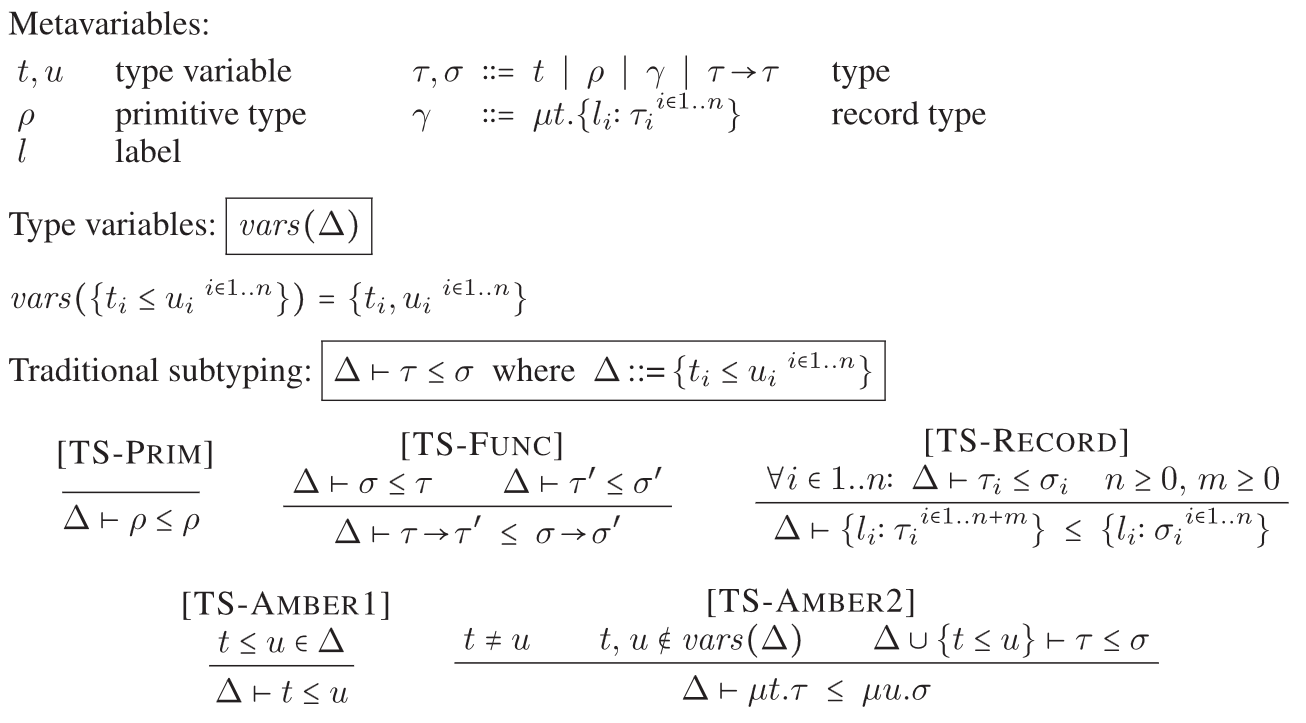
\includegraphics[height=0.85\textheight]{fig/subtyping1}
        \end{center}
    \end{frame}

    \begin{frame}{Пересмотренная подтипизация [\href{https://dl.acm.org/doi/pdf/10.1145/2888392}{Ryu et al, 2016}]}
        \begin{center}
            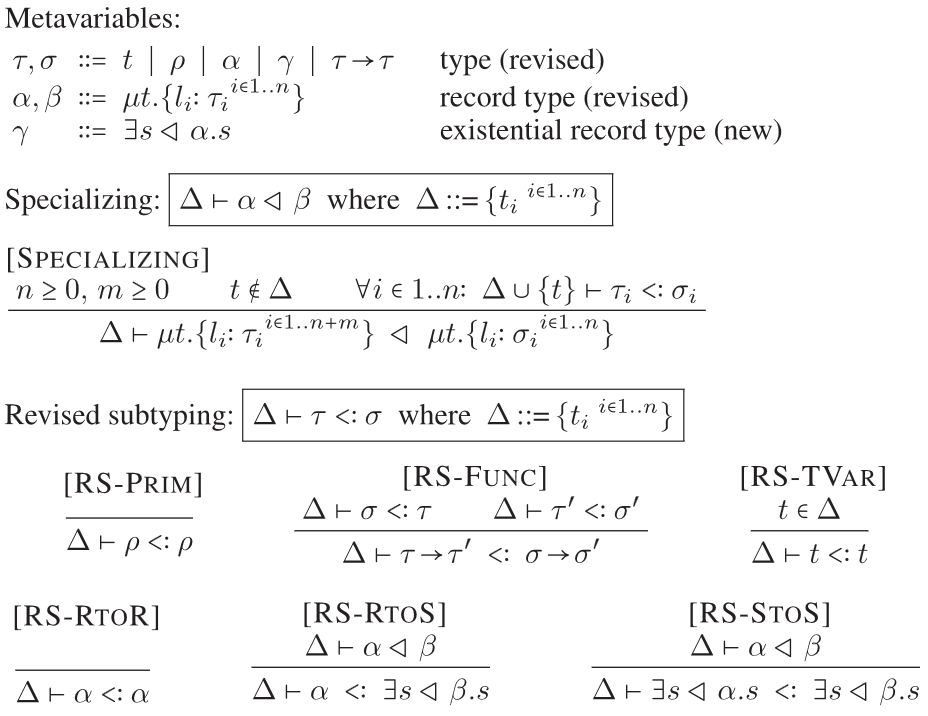
\includegraphics[height=0.85\textheight]{fig/subtyping2}
        \end{center}
    \end{frame}

    \begin{frame}{Соответствие правил для Kotlin с [\href{https://dl.acm.org/doi/pdf/10.1145/2888392}{Ryu et al, 2016}]}
        \begin{itemize}
            \item Self-тип --- это точный тип  $\mu t\ldotp \{ \overline{l_i : \tau_i} \}$ (exact type)
            \item А любой другой --- экзистенциальный тип $\exists s \triangleleft \alpha \ldotp s$ (inexact type)
        \end{itemize}

        \begin{block}{Подтипизация}
            Точный тип может быть подтипом экзистенциального, но не наоборот:
            \begin{columns}[onlytextwidth]
                \begin{column}[t]{0.485\textwidth}
                    \[
                        \infer[\text{RS-RtoS}]{
                            \Delta \vdash \alpha <: \exists s \triangleleft \beta \ldotp s
                        }{
                            \Delta \vdash \alpha \triangleleft \beta
                        }
                    \]
                \end{column}\hfill%
                \begin{column}[t]{0.485\textwidth}
                    \[
                        \infer[\text{Self-NoSelf}]{
                            \Delta \vdash Self(A) <: B
                        }{
                            \Delta \vdash A <: B
                        }
                    \]
                \end{column}
            \end{columns}
        \end{block}

        \begin{block}{Переписывание Self-типа}
            Переписывание сходно с одним шагом развёртки изорекурсивного типа:
            \vspace{-1em}
            \begin{columns}[onlytextwidth]
                \begin{column}[t]{0.41\textwidth}
                    \[
                        %! suppress = EscapeAmpersand
                        \infer[\text{Unfold-Self}]{
                            \Delta \vdash unfold(o) : [t \mapsto U]T
                        }{
                            U = \mu t \ldotp T & \Delta \vdash o : U
                        }
                    \]
                \end{column}\hfill%
                \begin{column}[t]{0.58\textwidth}
                    \[
                        %! suppress = EscapeAmpersand
                        \infer[\text{Unfold-NoSelf}]{
                            \Delta \vdash unfold(o) : [t \mapsto U']T
                        }{
                            U = \mu t \ldotp T
                            &
                            U' = \exists s \triangleleft U \ldotp s
                            &
                            \Delta \vdash o : U'
                        }
                    \]
                \end{column}
            \end{columns}
        \end{block}
    \end{frame}

    \begin{frame}[fragile]{Правила подтипизации для Self-типа}
        \begin{block}{Граница Self-типа}
            Тип $B$ является границей Self-типа (обозначение \underline{$Self(B)$}), если $B$~--- наиболее общий тип ресивера, на котором этот метод может быть вызван.
            Совпадает с типом текущего класса.
        \end{block}

        \begin{block}{Правила подтипизации для Self-типа}
            \begin{enumerate}
                \item \label{itm:covariant-bound} $B <: A \iff Self(B) <: Self(A)$ для возможности переопределения методов с \texttt{Self}
                \item \label{itm:this-subtype} $B <: A \iff Self(B) <: A$, чтобы код с \mintinline{kotlin}|this| оставался типизируемым
                \item \label{itm:any-nothing} $Nothing <: Self(A)$ и $Self(A) <: Any$
                \item \label{itm:no-subtypes} $B \bcancel{<:} Self(A)$, если $B$ не подходит под правила (\ref{itm:covariant-bound}) и (\ref{itm:any-nothing})
            \end{enumerate}
        \end{block}

        \begin{block}{Безопасность присваиваний}
            \begin{enumerate}
                \item \mintinline{kotlin}|this|, ссылающийся на ресивер $C$, имеет тип $Self(C)$
                \item Правило (\ref{itm:no-subtypes}) не позволяет использовать посторонний объект в качестве $Self$
            \end{enumerate}
        \end{block}
    \end{frame}

    \begin{frame}[fragile]{Некорректное создание новых объектов}
        \begin{columns}[onlytextwidth]
            \begin{column}[t]{0.46\textwidth}
                \vspace{0.5em}

                Для реализации персистентных и иммутабельных структур данных нужно иметь возможность создавать новый объект Self-типа.

                \vspace{1em}
                \begin{block}{В общем случае небезопасно}
                    \begin{itemize}
                        \item Создавать объект открытого класса
                        \item Создавать объект другого класса
                    \end{itemize}
                \end{block}
            \end{column}\hfill%
            \begin{column}[t]{0.50\textwidth}
                \begin{minted}[escapeinside=??]{kotlin}
                    open class A {
                        fun newOfOpenA(): Self = A()
                        fun newOtherQ(): Self = Q()
                    }

                    class Q : A() { fun qOnly() {} }
                    class P : A() { fun pOnly() {} }

                    fun test(q: Q, p: P) {
                        q.newOfOpenA() // скоуп типа Q для A
                         .qOnly()      // ?\err?
                        p.newOther()   // скоуп типа P для Q
                         .pOnly()      // ?\err?
                    }
                \end{minted}
            \end{column}
        \end{columns}
    \end{frame}

    \begin{frame}[fragile]{Безопасное создание новых объектов типа \texttt{Self(C)}}
        \begin{columns}[onlytextwidth]
            \begin{column}[t]{0.46\textwidth}
                \begin{block}{Ограничения}
                    \begin{itemize}
                        \item Класс \texttt{C} должен быть финальным
                        \item Тип \mintinline{kotlin}|this|\footnote{Ресивер текущей декларации (c типом bound'а Self-типа)} либо равен \texttt{С}, либо включает \texttt{C} после smart-cast
                        \item Тип \texttt{C} объявлен в том же модуле, в котором создаётся объект\footnote{Иначе открытие класса нарушало совместимость исходных кодов}
                    \end{itemize}
                \end{block}
            \end{column}\hfill%
            \begin{column}[t]{0.50\textwidth}
                \begin{minted}[escapeinside=??]{kotlin}
                    sealed interface Data {
                        data class One(var a: Int) : Data

                        data class Two(
                            var a: Int, var b: Int
                        ) : Data

                        fun copy(): Self = when (this) {
                            is One -> ?\colorbox{green}{One(a)}?   //: Self(One)
                            is Two -> ?\colorbox{green}{Two(a, b)}?//: Self(Two)
                        } // : Self(Data)
                    }
                \end{minted}
            \end{column}
        \end{columns}
    \end{frame}

    \begin{frame}[fragile]{Безопасность переписывания}
        \begin{enumerate}
            \item Значение Self-типа безопасно относительно переписывания
            \item Если ресивер имеет тип $A \neq Self$, \texttt{Self} переписывается в $A$, а $A \bcancel{<:} Self(A)$
            \item Если ресивер имеет тип \texttt{Self(B)}, то \texttt{Self(A)} декларации переписывается в \texttt{Self(B)}, и известно, что значение ресивера безопасно, материализуемое значение безопасно
        \end{enumerate}

        \begin{minted}{kotlin}
            abstract class A {
                fun self(): Self = this
                fun unsafeSelf(a: A): Self/*(A)*/ =
                    a    /* : A       */ .self() // : #\colorbox{yellow}{A}#, #\textcolor{red}{ошибка компиляции}#
                fun safeSelf():       Self/*(A)*/ =
                    this /* : Self(A) */ .self() // : #\colorbox{yellow}{Self(A)}#, ok, Self(A) <: Self(A)
            }
        \end{minted}
    \end{frame}


    \subsection{Реализация прототипа}

    \begin{frame}{Архитектура компилятора Kotlin (K2)}
        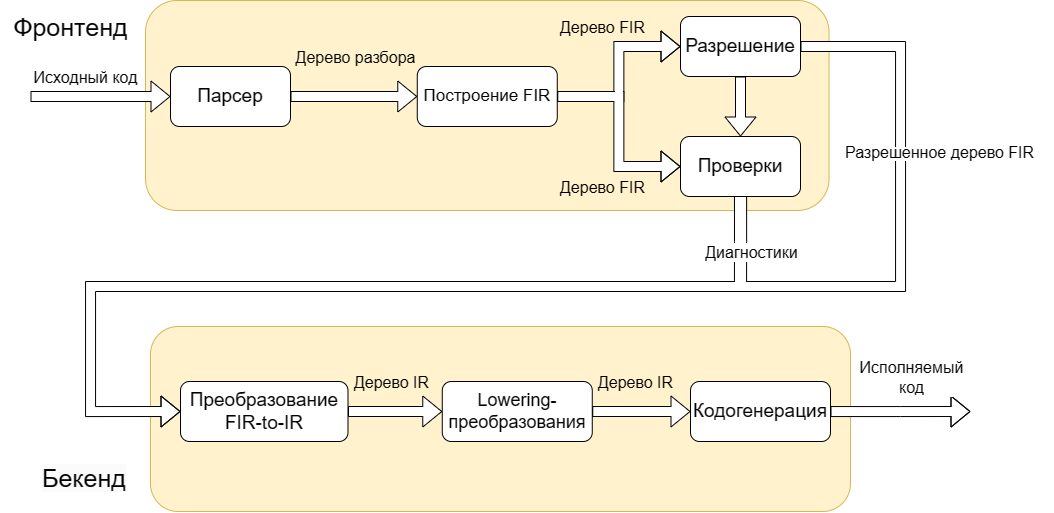
\includegraphics[width=\textwidth]{fig/arch}
    \end{frame}

    \begin{frame}{Детали реализации Self-типов в компиляторе kotlinc}
        \note{
            \begin{enumerate}
                \item Я реализовал прототип Self-типов в компиляторе kotlinc
                \item Для этого я:
                \begin{enumerate}
                    \item Дополнил правила типизации для работы с Self-типами
                    \item Реализовал область видимости, материализующую Self-тип
                    \begin{enumerate}
                        \item Для этого я генерирую для каждого места использования метода с Self-типом синтетическую декларацию
                        \item В будущем потребуется разработать более эффективную реализацию
                    \end{enumerate}
                    \item Также я протестировал полученную реализацию
                \end{enumerate}
            \end{enumerate}
        }

        \begin{enumerate}
            \item Идентификатор типа \texttt{Self} введён как ключевое слово языка
            \item Введён новый вид типов --- Self-типы
            \item Правила системы типов Kotlin доопределены для работы с Self-типами:
            \begin{itemize}
                \item Правило подтипизации
                \item Правило определения непосредственных супертипов
                \item Правило вычисления ближайших общих супертипов
            \end{itemize}
            \item Реализована область видимости\footnote{Области видимости --- сервисы компилятора, возвращающие множество функций, для которых объект данного типа может быть использован как получатель: $(plus : String\ldotp(String) \to String) \in scope(String)$}, переписывающая Self-тип
            \begin{itemize}
                \item Для каждого места вызова метода с Self-типом генерируется синтетическая декларация
                \item В будущем потребуется разработать более эффективную реализацию
            \end{itemize}
            \item Реализовано преобразование, подменяющее Self-тип на его границу и метаинформацию при переходе к промежуточному представлению бекенда компилятора (IR)
            \item Полученная реализация протестирована:
            \begin{itemize}
                \item Корректный код c Self-типами допускается системой типов
                \item Небезопасный код отвергается системой типов
            \end{itemize}
        \end{enumerate}
    \end{frame}

\end{document}
